\setchapterimage{bandeau}
\chapter*{Application \arabic{cptApplication} \\ 
Barrière sur la Tamise -- \ifprof Corrigé \else Sujet \fi}
\addcontentsline{toc}{section}{Application \arabic{cptApplication} : Barrière sur la Tamise -- \ifprof Corrigé \else Sujet \fi}

\iflivret \stepcounter{cptApplication} \else
\ifprof  \stepcounter{cptApplication} \else \fi
\fi

\setcounter{question}{0}
\marginnote{Florestan Mathurin.}
\marginnote{
\UPSTIcompetence[2]{B2-10}
}

%\begin{marginfigure}
%\centering
%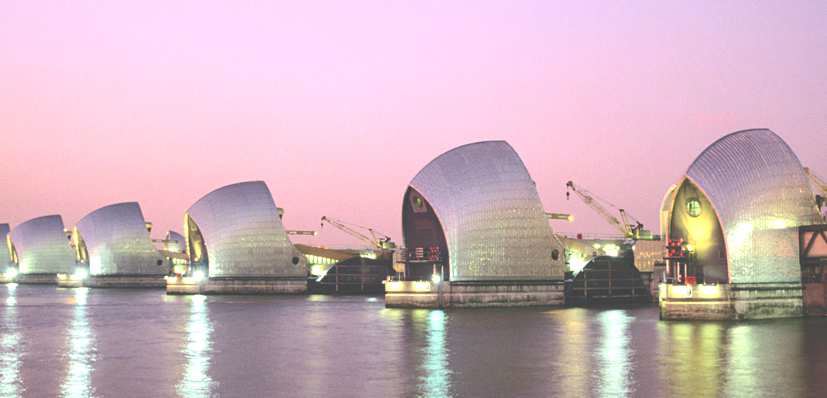
\includegraphics[width=4cm]{fig_00}
%\end{marginfigure}

%\section*{Barrière sur la Tamise}

Le barrage sur la Tamise permet de protéger Londres des grandes marrées évitant ainsi des crues qui pourraient survenir. Ce barrage est constituée de dix portes dont une modélisation est donnée ci-dessous.

\marginnote{On donne :
\begin{itemize}
\item $L=\SI{58}{m}$ la longueur de la porte;
\item $R=\SI{12,4}{m}$ le rayon de la porte;
\item $e=\SI{0,05}{m}$ l'épaisseur de la porte, considérée négligeable devant $R$;
\item $\rho=\SI{7800}{kg.m^{-3}}$;
\item $\alpha=\dfrac{\pi}{3}$.
\end{itemize}
}

\begin{center}
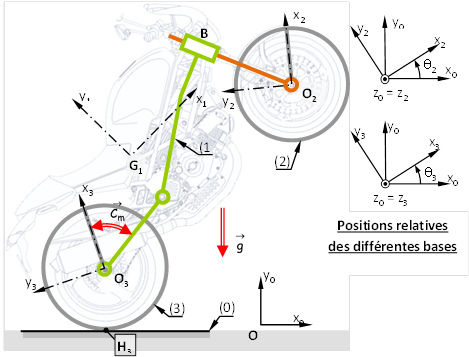
\includegraphics[width=10cm]{fig_01}
\end{center}


%\section*{Présentation du support du cours du cours}

\question{Déterminer les coordonnées du centre d'inertie de la porte : 
\begin{enumerate}
\item déterminer les coordonnées du centre d'inertie $G_P$ de la plaque;
\item déterminer les coordonnées du centre d'inertie $G_C$ de la portion cylindrique;
\item déterminer les coordonnées du centre d'inertie $G$ de la porte.
\end{enumerate}}

\ifprof
\begin{corrige}
\paragraph*{Coordonnées de $G_P$}

On a $\vect{OG_P}= -\cos\alpha \vy{} - \dfrac{L}{2} \vz{}$.

\paragraph*{Coordonnées de $G_C$}

Pour des raisons de symétrie, on a $\vect{OG_C}= Y_{C} \vy{} - \dfrac{L}{2} \vz{}$.

Par définition, on a alors $m_c Y_{C} = \int y_p \text{d} m$.

On a, en coordonnées cylindriques, $Y_p =- R\cos\theta$, $\text{d} m = \rho L R \text{d} \theta$ avec $\theta$ variant de $-\alpha$ à $\alpha$.

Par suite, $m_c Y_{C} = -\int\limits_{-\alpha}^{\alpha} R \cos \theta  \rho L R \text{d} \theta$ 
$=-\rho R^2 L\left[\sin \theta \right]_{-\alpha}^{\alpha}$
$=-2\rho R^2 L  \sin\alpha$. 

Or, $m_c = 2R\alpha L \rho$. En conséquences, $2R\alpha L \rho Y_{C}=-2 L \rho R^2  \sin\alpha$ et 
$ Y_{C}=- R  \dfrac{\sin\alpha}{\alpha}$. 
%
%
\paragraph*{Coordonnées de $G$}

En utilisant la définition du barycentre, on a $m \vect{OG} = m_P \vect{OG_P}+m_C \vect{OG_C}$.
\end{corrige}
\else

\fi


\question{Déterminer la forme de la matrice d'inertie de la porte :
\begin{enumerate}
\item donner la forme de la matrice d'inertie de la plaque $P$ en $G_P$;
\item donner la forme de la matrice d'inertie du cylindre $C$ en $G_C$;
\item donner la forme de la matrice d'inertie de la porte $P$ en $G$.
\end{enumerate}}

\question{Déterminer la moment d'inertie de la porte par rapport à $\axe{O}{z}$.}

%
%\ifprof
%\else
%
%
%\fi
%
%\newpage
%
%\section*{Matrices d'inertie}
%\subparagraph*{}\textit{Donner les formes des matrices d'inertie suivantes.}
%
%\begin{center}
%\begin{tabular}{|c|p{2cm}||c|p{2cm}|}
%\hline 
%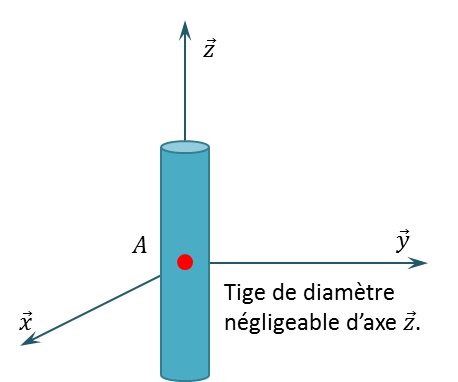
\includegraphics[width=2.8cm]{qcm/Fig_01} & & 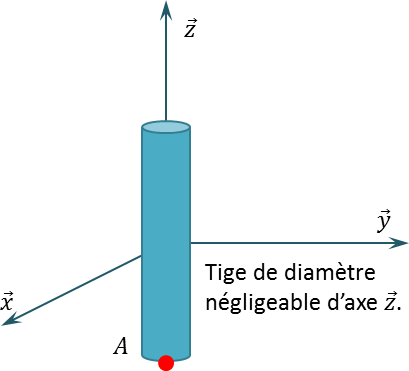
\includegraphics[width=2.8cm]{qcm/Fig_02} & \\ \hline
%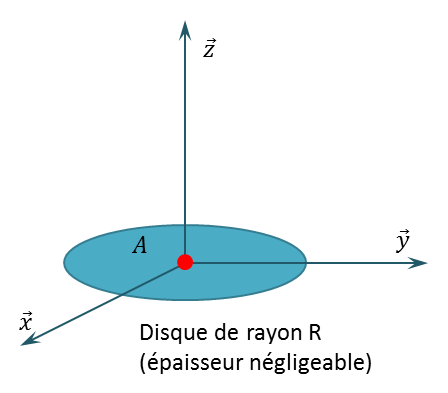
\includegraphics[width=2.8cm]{qcm/Fig_04} & & 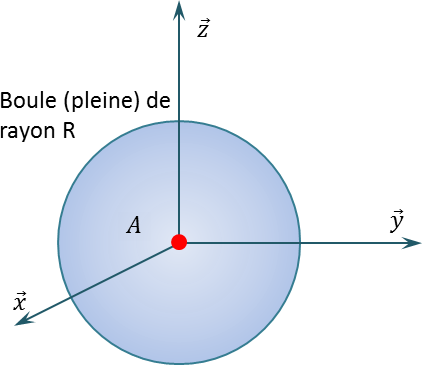
\includegraphics[width=2.8cm]{qcm/Fig_05} & \\ \hline
%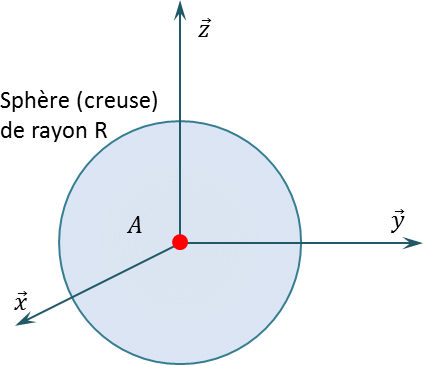
\includegraphics[width=2.8cm]{qcm/Fig_06} & & 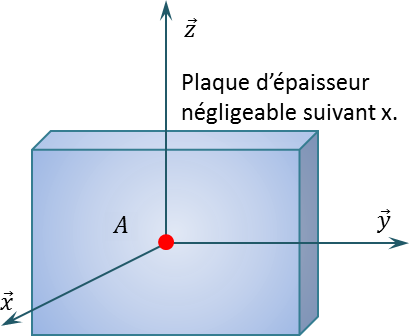
\includegraphics[width=2.8cm]{qcm/Fig_07} & \\ \hline
%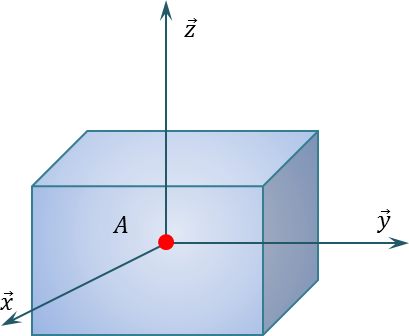
\includegraphics[width=2.8cm]{qcm/Fig_08} & & 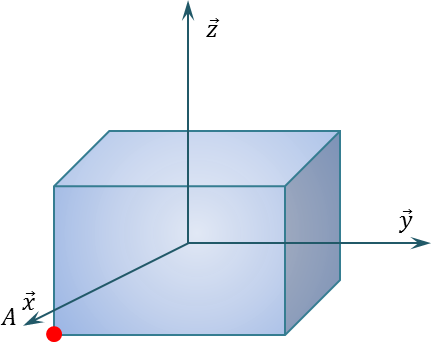
\includegraphics[width=2.8cm]{qcm/Fig_09} & \\ \hline
%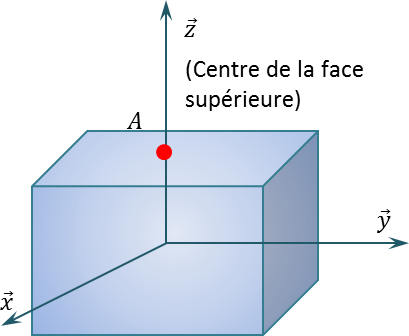
\includegraphics[width=2.8cm]{qcm/Fig_10} & & 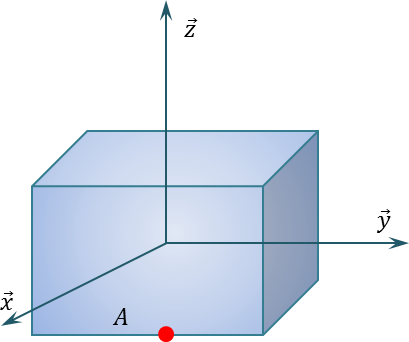
\includegraphics[width=2.8cm]{qcm/Fig_11} & \\ \hline
%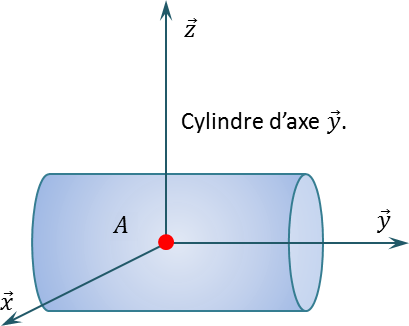
\includegraphics[width=2.8cm]{qcm/Fig_12} & & 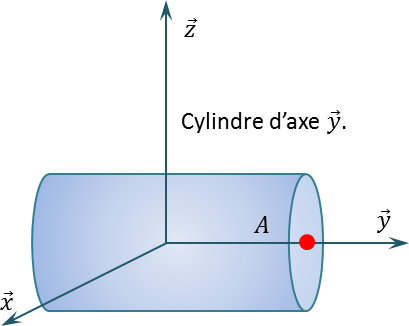
\includegraphics[width=2.8cm]{qcm/Fig_13} & \\ \hline
%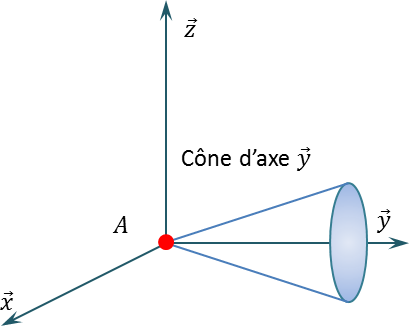
\includegraphics[width=2.8cm]{qcm/Fig_14} & & 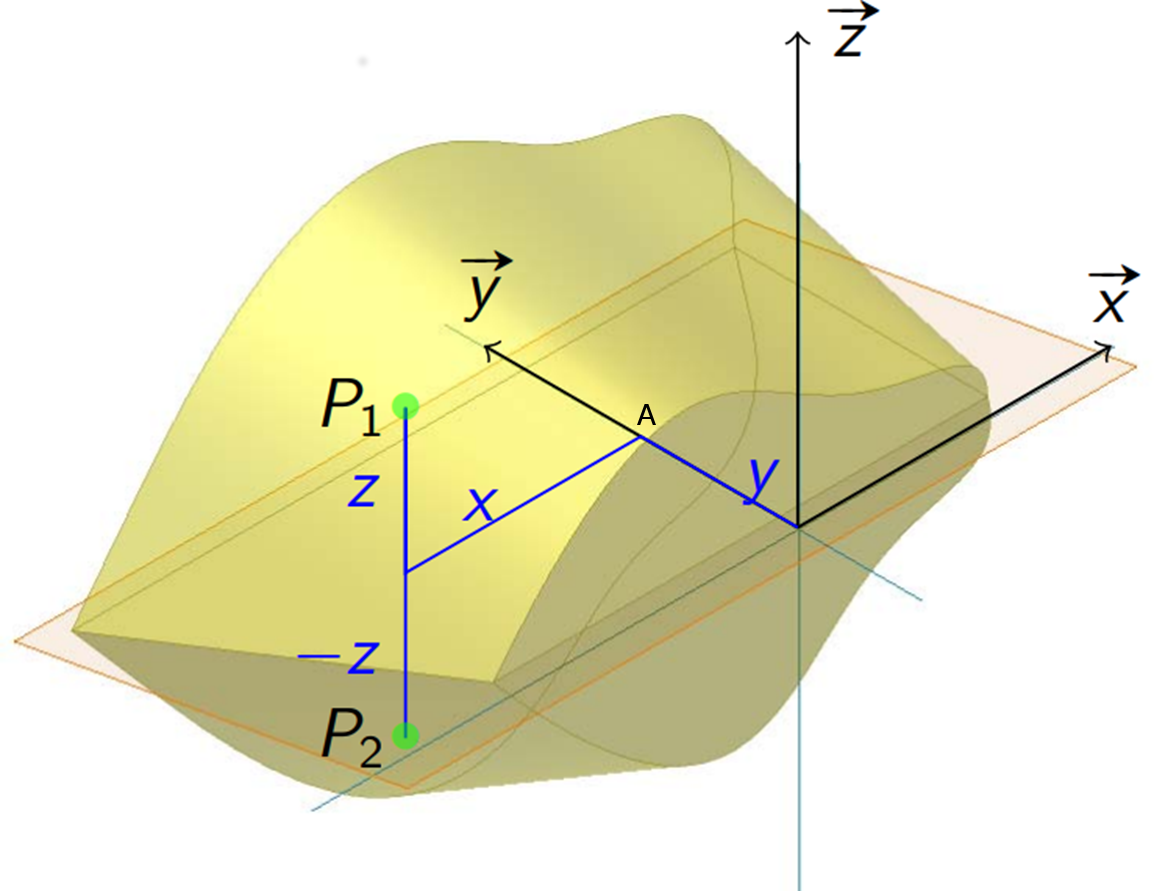
\includegraphics[width=2.8cm]{qcm/Fig_15} & \\ \hline
%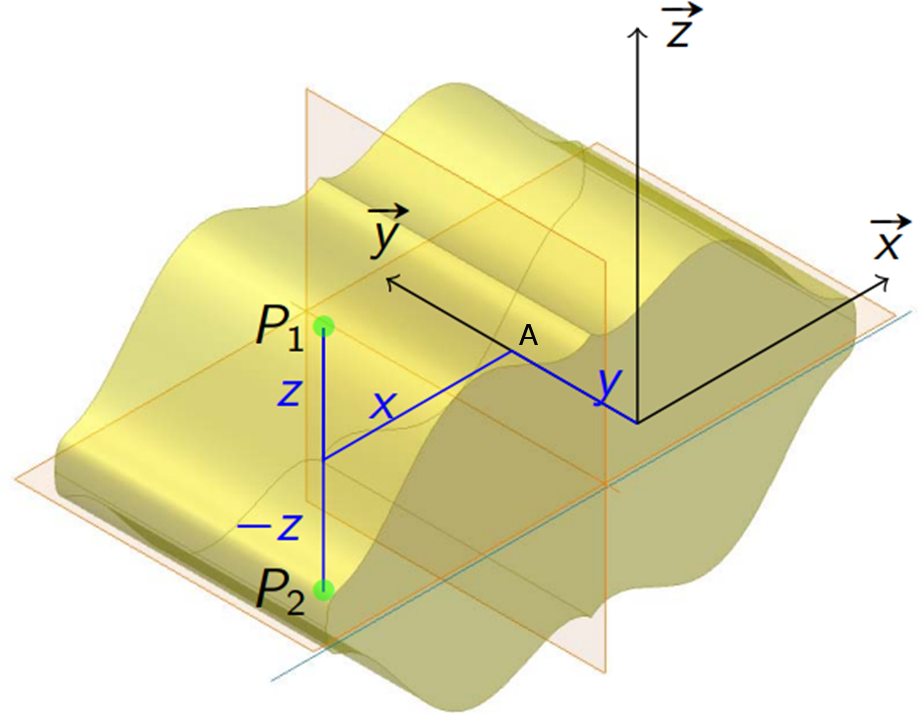
\includegraphics[width=2.8cm]{qcm/Fig_16} & & 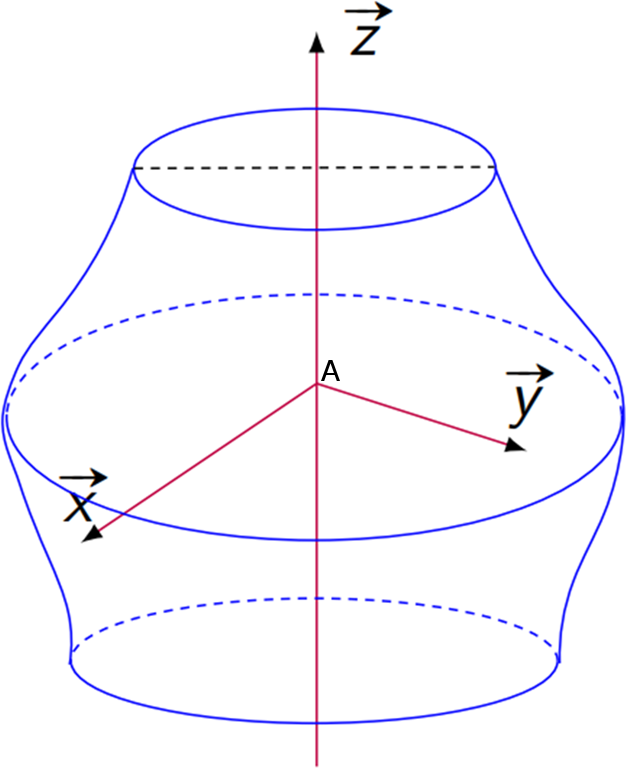
\includegraphics[width=2.8cm]{qcm/Fig_17} & \\ \hline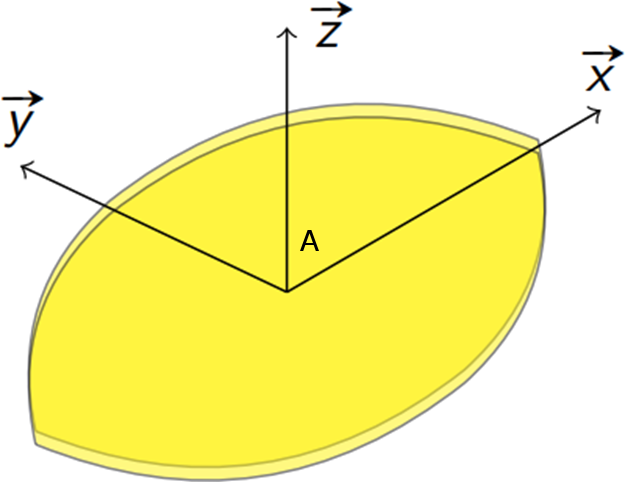
\includegraphics[width=2.8cm]{qcm/Fig_18} & &  & \\ \hline
%\end{tabular}
%\end{center}

